\documentclass[12pt]{iptex}
% IDIOMA
% Se necessário, inserir línguas e indicar língua principal (main)
\usepackage[main=brazil,english]{babel}
\usepackage[italic]{mathastext}
\sisetup{
    group-separator={.},
    group-minimum-digits=3,
    output-decimal-marker={,}}

% Alterando nome do TOC (adicionar em outras línguas, se necessário)
\addto\captionsbrazil{%
	\renewcommand{\contentsname}{SUMÁRIO}
	\renewcommand{\refname}{REFERÊNCIAS}
}

% BIBLIOGRAFIA
%\usepackage[abnt-emphasize=bf,alf]{abntex2cite}
% Para bibliografia ABNT com números
\usepackage[abnt-emphasize=bf,num]{abntex2cite}
\citebrackets[]

% Para outros estilos o autor deve definir o \bibliographystyle dentro do documento

% Início do documento
\begin{document}

% CAPA 
% Params
\tipo{BOLETIM SISMOLÓGICO}
\data{2023}

\titulo{Estação Sismológica SP7, SC \\
          UHE Machadinho SC/RS \\
          BOLETIM SÍSMICO Nº 26/36-2024 Ago.23 }

\unidade{Cidades Infraestruturas e Meio Ambiente}{CIMA}
\lab{Seção de Obras Civis - SOC}
\periodo{01/08/2023}{31/08/2023}

% Inserir capa
\capa
\pagestyle{timbrado}

\vspace{0.5cm}

\pagestyle{geral}


% Corpo
\pagestyle{geral}
% Corpo do documento
\section{ÚLTIMOS RELATÓRIOS TÉCNICOS}
\label{sec:ultimos_relatorios}
\begin{itemize}
    \item Relatório IPT Nº 169 991-205 - "Análise dos registros obtidos entre 01 de dezembro de 2022 e 30 de junho de 2023 na estação Sismológica SP7, Salto Pilão, SC.", emitido em agosto de 2023. 
\end{itemize}

\section{ATIVIDADES REALIZADAS}
\label{sec:atividade}
\begin{itemize}
    \item Encaminhamento do boletim sísmico nº 26/36-2024, Agosto-2023;
    \item Coleta de dados em 21/09/2023 e envio dos mesmos para análise no IPT;
    \item Processamento preliminar dos dados do período (01/08/2023 a 31/08/2023), referente às coletas SP723230 (05/07/2023 a 18/08/2023) e SP723264 (18/08/2023 a 21/09/2023); 
    \item Elaboração do gráfico de completeza dos dados, tabela contendo os registros de eventos/detonações detectados e mapa da região indicando os epicentros localizados;
	\item  Comparação dos desmontes detectados aos planos de fogo das pedreiras Azza e Daclande.
\end{itemize}

\section{RESULTADOS}
\label{sec:resultados}
\begin{itemize}
	\item A análise preliminar dos dados mostrou que a estação SP7 teve funcionamento normal e satisfatório durante o período de análise deste boletim sísmico (18/08/2023 a 21/09/2023). O gráfico de completeza para o período é mostrado na Figura 1. 
    \item Foram detectados quinze desmontes na área do entorno do empreendimento durante o período, sendo três na região das pedreiras Azza e Daclande (sem confirmação pelo plano de fogo das pedreiras) e os restantes localizados em outras pedreiras/áreas de mineração identificadas por imagens de satélite. O maior desmonte detectado no período teve magnitude 1.8 MLv e foi detectado em 2023-08-21 20:32:38 (UTC), longe da região do reservatório. O desmonte foi assim classificado por sua forma de onda sísmica, epicentro, horário de ocorrência e magnitude. 
    \item Durante o período não foram detectados sismos naturais locais, regionais e/ou telessismos em território brasileiro pela estação SP7. 
    \item Os parâmetros epicentrais dos eventos se encontram detalhados na Tabela 1. O mapa de entorno da região junto da localização dos epicentros é mostrado na Figura 2. 
\end{itemize}
    

\section{CONSIDERAÇÕES}
\label{sec:consideracoes}
Continuam válidas as considerações e orientações anteriores a respeito das medidas a serem tomadas em caso ocorrência de um sismo local sentido pela população, i.e., coletar os relatos da população local através de questionários macrossísmicos, contactar a defesa civil para avaliar possíveis danos em estruturas e fornecer orientações e informações à população. 

\assinaturaLucas
\clearpage
\newpage


\section{COMPLETUDE DOS DADOS}

\begin{figure}[htb!]
    \centering
	\captionsetup{justification=raggedright, singlelinecheck=false, width=1\textwidth}
    \caption{Gráfico de completude dos dados para o mês de agosto/2023 para a estação SP7.}
    \begin{mdframed}[
        linecolor=black,
        linewidth=1pt,
        roundcorner=10pt,
    ]
    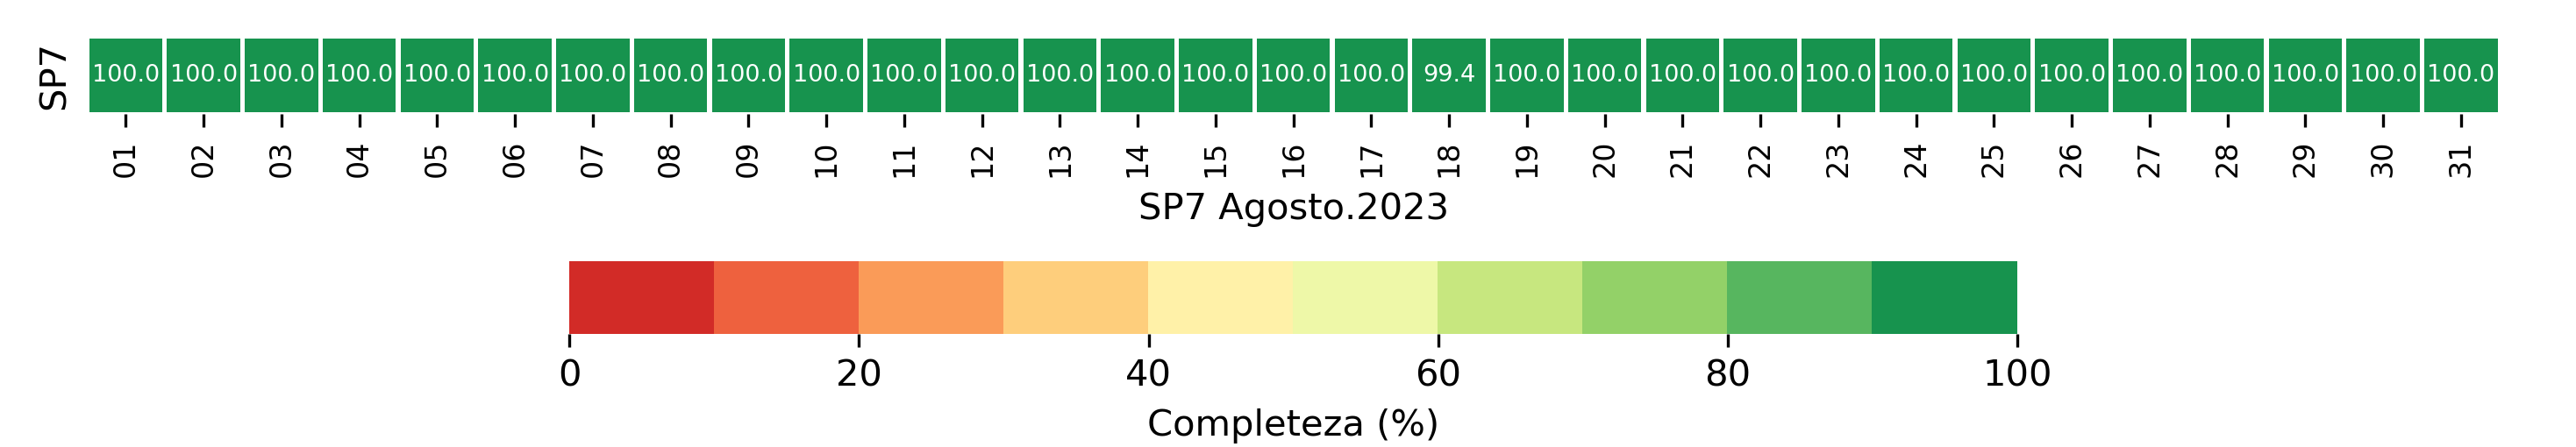
\includegraphics[width=1.0\textwidth]{./boletim/salto_pilao/figuras/completude_SP7.png} % Substitua pelo nome da imagem e ajuste o tamanho
    %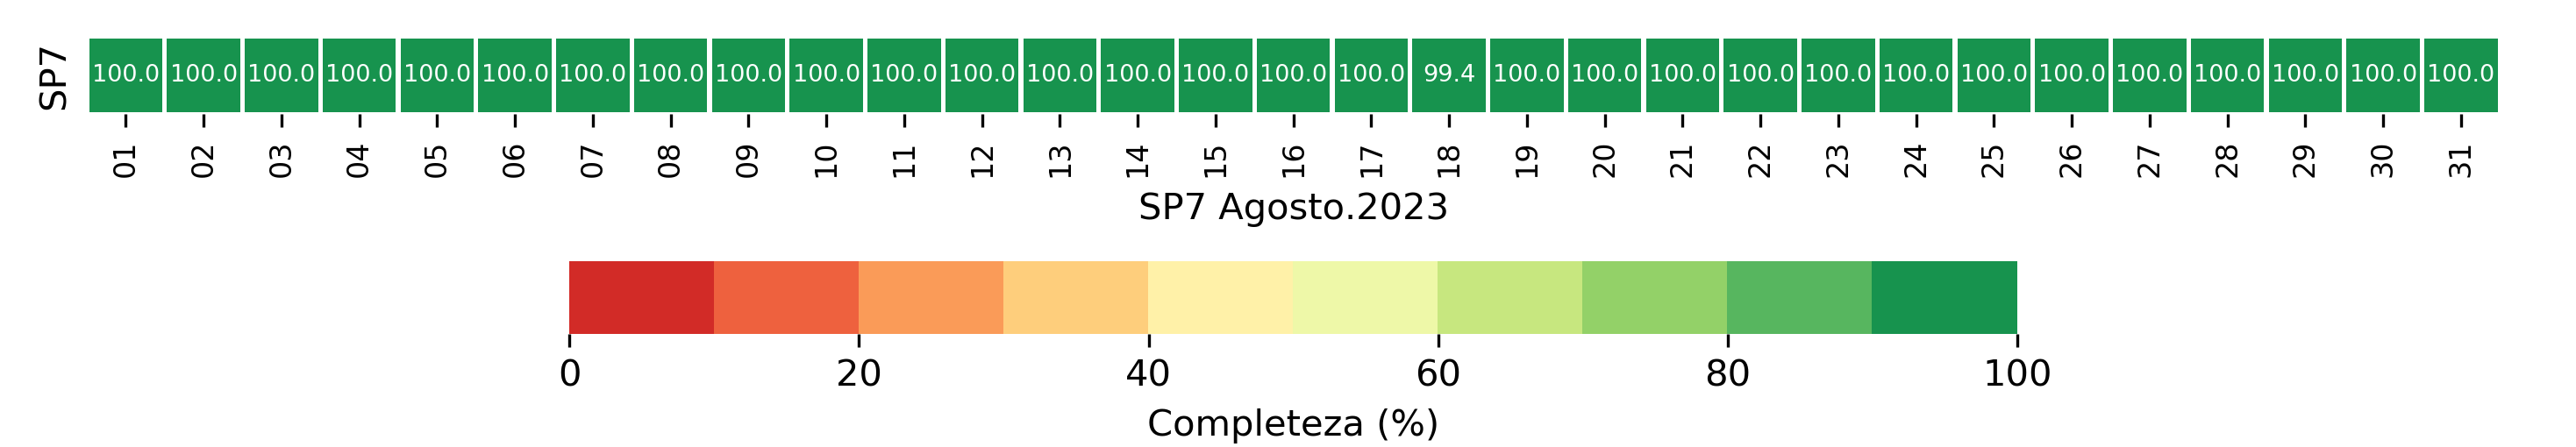
\includegraphics[width=1.0\textwidth]{./boletim/salto_pilao/figuras/completude_SP7.png}
    \end{mdframed}
    \caption*{Fonte: IPT}
    \label{fig:completude}
\end{figure}



\section{TABELA DE EVENTOS}
\begin{center}
\scriptsize
\setlength{\arrayrulewidth}{0.05pt}
\begin{longtable}{ccccS[table-format=6.0]S[table-format=7.0]ccc}
\captionsetup{justification=justified,singlelinecheck=false}
\caption{Listagem de eventos detectados e categorizados durante o período de interesse.\\ A coluna \textit{Cat} representaria a categoria na qual o evento foi classificado sendo \textit{Q} = Detonação/Desmontes, \textit{E} = Sismo Regional e \textit{I} = Sismo induzido e \textit{N} = Não-localizável. O valor da energia para os sismos foi obtido a partir da magnitude através da relação proposta por Richter (1958). Fonte: IPT.}\\
%%%%%%%%%%%%%%%%%%%%%%%%%%%%%%%%%%%%%%%%%%%%%%%%%%%%%%%
\hline \\[-4ex]
\hline \\[-5ex]
\multicolumn{1}{c}{ID} &
\multicolumn{1}{c}{Hora de Origem (UTC)} &
\multicolumn{1}{c}{Longitude} &
\multicolumn{1}{c}{Latitude} &
\multicolumn{1}{c}{UTM X} &
\multicolumn{1}{c}{UTM Y} &
\multicolumn{1}{c}{MLv} &
\multicolumn{1}{c}{Energia} &
\multicolumn{1}{c}{Cat} \\


\\[-5.0ex] \hline
\\[-5.0ex]

\multicolumn{1}{c}{\textit{{}}} & 
\multicolumn{1}{c}{\textit{{}}} & 
\multicolumn{1}{c}{\textit{(\textdegree\hspace{0.25em})}} & 
\multicolumn{1}{c}{\textit{(\textdegree\hspace{0.25em})}} & 
\multicolumn{1}{c}{\textit{{(m)}}} & 
\multicolumn{1}{c}{\textit{{(m)}}} & 
\multicolumn{1}{c}{\textit{{}}} & 
\multicolumn{1}{c}{\textit{{(J)}}} & 
\multicolumn{1}{c}{\textit{{}}} \\ 

\\[-5.0ex] \hline
\\[-4.0ex]
\endfirsthead


%%%%%%%%%%%%%%%%%%%%%%%%%%%%%%%%%%%%%%%%%%%%%%%%%%%%%%%
\hline \\[-4ex]
\hline \\[-5ex]
\multicolumn{1}{c}{ID} &
\multicolumn{1}{c}{Hora de Origem (UTC)} &
\multicolumn{1}{c}{Longitude} &
\multicolumn{1}{c}{Latitude} &
\multicolumn{1}{c}{UTM X} &
\multicolumn{1}{c}{UTM Y} &
\multicolumn{1}{c}{MLv} &
\multicolumn{1}{c}{Energia} &
\multicolumn{1}{c}{Cat} \\


\\[-5.0ex] \hline
\\[-5.0ex]

\multicolumn{1}{c}{\textit{{}}} & 
\multicolumn{1}{c}{\textit{{}}} & 
\multicolumn{1}{c}{\textit{(\textdegree\hspace{0.25em})}} & 
\multicolumn{1}{c}{\textit{(\textdegree\hspace{0.25em})}} & 
\multicolumn{1}{c}{\textit{{(m)}}} & 
\multicolumn{1}{c}{\textit{{(m)}}} & 
\multicolumn{1}{c}{\textit{{}}} & 
\multicolumn{1}{c}{\textit{{(J)}}} & 
\multicolumn{1}{c}{\textit{{}}} \\

\\[-5.0ex] \hline
\\[-4.0ex]
\endhead
\hline
\caption*{Fonte: IPT.}

\endlastfoot
%%%%%%%%%%%%%%%%%%%%%%%%%%%%%%%%%%%%%%%%%%%%%%%%%%%%%%%
SP\_20230830\_204938 & 2023-08-30T20:49:38 & -49,1929 & -27,2837 & 678857 & 6980853 & 1,7 & \num[round-precision=3,round-mode=figures,scientific-notation=true]{1.25027e+06} & Q \\
SP\_20230824\_152929 & 2023-08-24T15:29:29 & -49,3706 & -27,3787 & 661127 & 6970564 & 1,6 & \num[round-precision=3,round-mode=figures,scientific-notation=true]{965367} & Q \\
SP\_20230824\_144552 & 2023-08-24T14:45:52 & -49,5194 & -27,0966 & 646786 & 7002001 & 1,4 & \num[round-precision=3,round-mode=figures,scientific-notation=true]{306963} & Q \\
SP\_20230821\_203238 & 2023-08-21T20:32:38 & -49,5775 & -27,3768 & 640663 & 6971026 & 1,8 & \num[round-precision=3,round-mode=figures,scientific-notation=true]{2.2464e+06} & Q \\
SP\_20230818\_154946 & 2023-08-18T15:49:46 & -49,3619 & -27,3734 & 661995 & 6971146 & 1,1 & \num[round-precision=3,round-mode=figures,scientific-notation=true]{82923.6} & Q \\
SP\_20230818\_154759 & 2023-08-18T15:47:59 & -49,3671 & -27,3769 & 661476 & 6970762 & 1,7 & \num[round-precision=3,round-mode=figures,scientific-notation=true]{1.24523e+06} & Q \\
SP\_20230818\_152819 & 2023-08-18T15:28:21 & -49,4774 & -26,8329 & 651297 & 7031160 & 1,5 & \num[round-precision=3,round-mode=figures,scientific-notation=true]{464046} & Q \\
SP\_20230818\_152821 & 2023-08-18T15:28:21 & -49,4774 & -26,8329 & 651297 & 7031160 & 1,5 & \num[round-precision=3,round-mode=figures,scientific-notation=true]{464022} & Q \\
SP\_20230816\_200712 & 2023-08-16T20:07:12 & -49,1595 & -27,2413 & 682234 & 6985502 & 1,1 & \num[round-precision=3,round-mode=figures,scientific-notation=true]{85169.1} & Q \\
SP\_20230816\_184633 & 2023-08-16T18:46:33 & -49,5424 & -27,0343 & 644578 & 7008934 & 1,3 & \num[round-precision=3,round-mode=figures,scientific-notation=true]{208955} & Q \\
SP\_20230815\_152857 & 2023-08-15T15:28:57 & -49,3792 & -27,3807 & 660279 & 6970351 & 1,6 & \num[round-precision=3,round-mode=figures,scientific-notation=true]{1.03504e+06} & Q \\
SP\_20230809\_173435 & 2023-08-09T17:34:35 & -48,9411 & -26,9649 & 704364 & 7015787 & 1,7 & \num[round-precision=3,round-mode=figures,scientific-notation=true]{1.11257e+06} & Q \\
SP\_20230808\_153702 & 2023-08-08T15:37:02 & -49,3712 & -27,3758 & 661069 & 6970883 & 1,2 & \num[round-precision=3,round-mode=figures,scientific-notation=true]{121291} & Q \\
SP\_20230803\_175815 & 2023-08-03T17:58:15 & -49,5190 & -27,0966 & 646823 & 7002004 & 1,5 & \num[round-precision=3,round-mode=figures,scientific-notation=true]{555230} & Q \\
SP\_20230801\_181710 & 2023-08-01T18:17:10 & -49,3781 & -27,3687 & 660402 & 6971680 & 1,6 & \num[round-precision=3,round-mode=figures,scientific-notation=true]{821247} & Q \\
\end{longtable}
\end{center}



    \newpage
    \section{Mapa de eventos}
    \begin{figure}[ht!]
    \centering
    \captionsetup{justification=justified, singlelinecheck=false, width=1\textwidth}
    \caption{Mapa da região de interesse no entorno do empreendimento, mostrando as principais cidades, rodovias e rios, com a localização das pedreiras, estações \textbf{BCM2} e \textbf{MC9}, e eventos próximos ao empreendimento detectados no período de interesse.}
    \begin{mdframed}[
        linecolor=black,
        linewidth=1pt,
        roundcorner=10pt,
    ]
    \begin{center}
    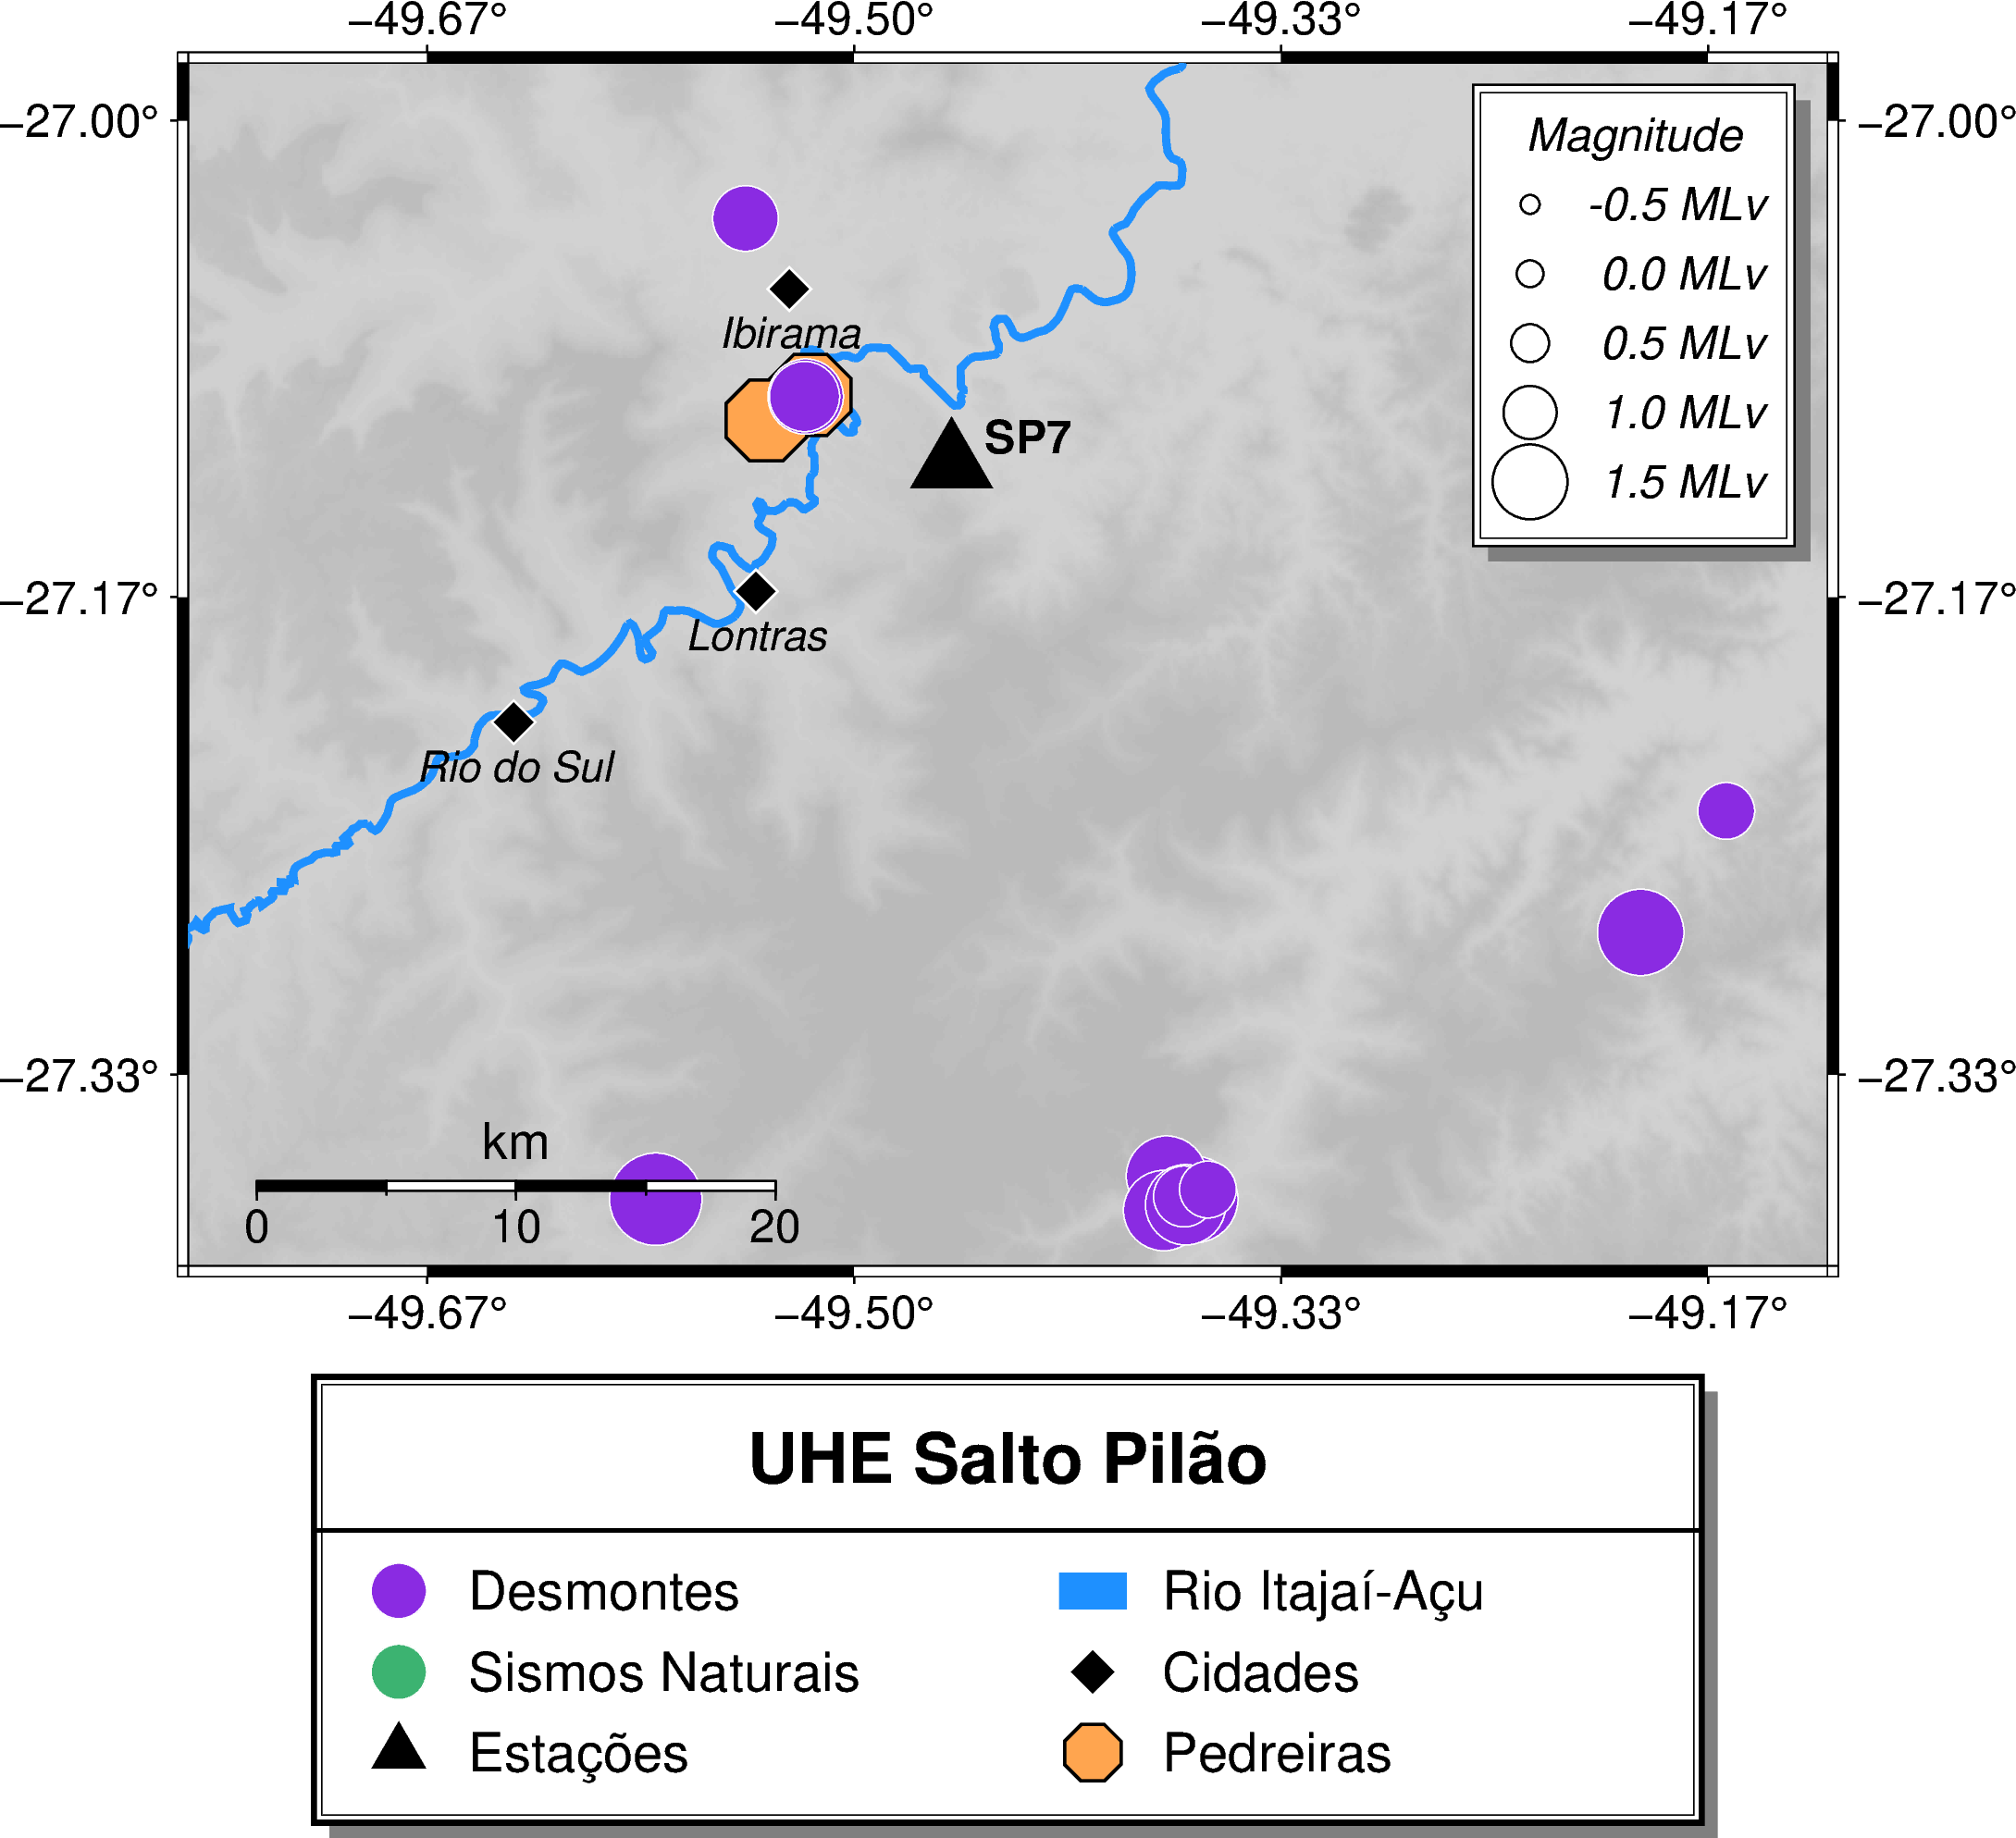
\includegraphics[width=1.0\textwidth]{./boletim/salto_pilao/figuras/mapaevents.png}
    \end{center}
    \end{mdframed}
    \caption*{Fonte: IPT}
    \end{figure}
    \newpage
    

% Bibliografia
\clearpage
\section{REFERÊNCIAS BIBLIOGRÁFICAS}

C. F. RICHTER, \textit{Elementary Seismology}, W. H. Freeman and Co., San Francisco, 1958, 768 pp.
%\renewcommand{\refname}{REFERÊNCIAS}
%\addcontentsline{toc}{section}{REFERÊNCIAS}
%\bibliography{ref}

\end{document}
